\documentclass{article}
\usepackage[utf8]{inputenc}
\usepackage{amsmath}
\usepackage{amsfonts}
\usepackage{amssymb}
\usepackage{graphicx}
\usepackage{listings}
\usepackage{xcolor}
\usepackage{minted}
\usepackage{biblatex}
\addbibresource{references.bib}

\title{ABC - Approximate Bayesian Computation}
\author{Max Lang}
\date{}
\begin{document}
\maketitle


\section{Why do we need ABC and why is it useful?}
ABC is particularly useful when dealing with complex models where the likelihood function is difficult or impossible to calculate. To understand its significance, let's delve into a worked example where normal methods do not suffice, and the application of ABC becomes invaluable.

This commonly arises in two main settings.
\begin{enumerate}
    \item Un-normalised likelihood: the observation model is given in the form
$$
p\left(y_{o b s} \mid \theta\right)=p\left(y_{o b s}, \theta\right) / c(\theta)
$$
with
$$
c(\theta)=\int_y p(y, \theta) d y
$$
and\textbf{ $c(\theta)$ may be intractable}. However we sometimes also encounter \textbf{intractable priors}.
\item Likelihood free: Sometimes the \textbf{observation model is not defined by a density at all, just a complex simulator }- essentially a piece of code that takes as input a parameter $\theta$ and some random variables $Z$ with the same dimension as $Y$ and returns as output a simulated realisation of $Y$. Although $p\left(y_{o b s} \mid \theta\right)$ is formally defined by the simulator, we have no idea what the function $p(y \mid \theta)$ actually is and how it depends on $\theta$. This appears alot in big physics based models including some climate models. \cite{martin_bayesian_2022}
\end{enumerate}



\subsection{Worked Example: When Normal Methods Fail and ABC Shines}
Consider a scenario in data analysis where we need to estimate parameters of a statistical model, but the likelihood function, which is central to Bayesian inference, is either too complex or unknown. Traditional methods like Maximum Likelihood Estimation (MLE) or standard Bayesian approaches hinge on the ability to calculate this likelihood, which might be unfeasible in many real-world situations.

\subsubsection{Ising Model}
Denote by $\mathcal{Y}=\{0,1\}^{m^2}$ the set of all binary $m \times m$ "images" $Y=$ $\left(Y_1, Y_2, \ldots, Y_{m^2}\right), Y_i \in\{0,1\}$, where $i=1,2, \ldots, m^2$ is the cell or "pixel" index in the square lattice of image cells. We say two cells $i$ and $j$ are neighbors and write $i \sim j$ if the cells share an edge in
\begin{table}[]
    \centering
    \begin{tabular}{|l|l|l|}
\hline 1 & 2 & 3 \\
\hline 4 & 5 & 6 \\
\hline 7 & 8 & 9 \\
\hline

\end{tabular}
    \caption{Cell index labels in a $3 \times 3$ square lattice}
    \label{tab:ising-1}
\end{table}



\begin{table}
    \centering
\begin{tabular}{|l|l|l|}
\hline 0 & 0 & 1 \\
\hline 0 & 1 & 1 \\
\hline 0 & 1 & 1 \\
\hline
\end{tabular}
    \caption{Possible realisation of the Ising model}
    \label{tab:ising-2}
\end{table}


 For example $5 \sim 6$ in Table \ref{tab:ising-1} and the neighbors of cell 9 are $\{8,6\}$. Let
$$
\# y=\frac{1}{2} \sum_{i=1}^{m^2} \sum_{j \sim i} \mathbb{I}_{Y_j \neq Y_i}
$$
where $\sum_{j \sim i}$ sums over all $j$ such that $j$ is a neighbor of $i$. Here \#y counts the number of "disagreeing neighbors" in the binary image $Y=y$. In the example in Table \ref{tab:ising-1} we have \#y=4.

\textbf{The Ising model with a free boundary is the following distribution over $\mathcal{Y}$ :}
$$
p(y \mid \theta)=\exp (-\theta \# y) / c(\theta) .
$$

It has a free boundary because cells on the edge have no neighbors beyond the edge. Here $\theta \geq 0$ is a positive smoothing parameter and
$$
c(\theta)=\sum_{y \in \mathcal{Y}} \exp (-\theta \# y)
$$
is \textbf{a normalizing constant which we cant compute for $n$ large}. There are $2^{m^2}$ terms in the sum, and no one can solve it (it is an important model in physics, so many have looked at this).

Suppose we have image data $Y=y_{o b s}$ with $y_{o b s} \in\{0,1\}^{m^2}$ and we want to estimate $\theta$. Consider doing MCMC targeting $\pi\left(\theta \mid y_{o b s}\right)$ with some prior $\pi(\theta)$. Choose a simple proposal for the scalar parameter $\theta$, say $\theta^{\prime} \sim U(\theta-a, \theta+a), a>0$. The acceptance probability is
$$
\begin{aligned}
\alpha\left(\theta^{\prime} \mid \theta\right) & =\min \left\{1, \frac{p\left(y \mid \theta^{\prime}\right) \pi\left(\theta^{\prime}\right)}{p(y \mid \theta) \pi(\theta)}\right\} \\
& =\min \left\{1, \frac{c(\theta)}{c\left(\theta^{\prime}\right)} \times \exp \left(\left(\theta-\theta^{\prime}\right) \# y\right) \times \frac{\pi\left(\theta^{\prime}\right)}{\pi(\theta)}\right\}
\end{aligned}
$$
and although $p(y)$ cancels,\textbf{ $c(\theta) / c\left(\theta^{\prime}\right)$ does not, and so we are left with an acceptance probability we cannot evaluate.} This leads us to the following definition.


\subsection{Doubly Intractable Distributions}

Doubly intractable distributions present a significant challenge in statistical computing, primarily encountered in Bayesian analysis. These distributions are characterized by a likelihood function that includes an intractable normalizing constant, which itself depends on the parameters of interest. This dependency creates a 'double' intractability: not only is the likelihood intractable, but so is its normalization.
\newline
\textbf{Definition 3.2.} (doubly intractable problems) If for $y_{o b s} \in \mathcal{Y}$ and $\theta, \theta^{\prime} \in \Omega$ either of the ratios $p\left(y_{o b s} \mid \theta\right) / p\left(y_{o b s} \mid \theta^{\prime}\right)$ or $\pi(\theta) / \pi\left(\theta^{\prime}\right)$ cannot be evaluated then the posterior is said to be doubly intractable.

ABC provides a pathway to handle these doubly intractable problems. By comparing simulated and observed data without the need to directly calculate the likelihood or its normalizing constant. 

\section{Main Concepts and Idea of Approximate Bayesian Computation (ABC)}
The cornerstone of ABC is its departure from the conventional reliance on the likelihood function in Bayesian inference. In many statistical models, especially those arising in biological, ecological, and physical sciences, the likelihood function can be so complex or computationally demanding that it becomes a bottleneck. ABC circumvents this by not requiring the explicit calculation of the likelihood. Instead, it \textbf{focuses on the similarity between observed data and data generated by the model}, using this comparison to infer model parameters.
\subsection{Goal of ABC:  Approximating the Approximated Posterior.}
In ABC, the goal is to approximate the posterior distribution of the parameters, which in traditional Bayesian analysis would be derived using Bayes' theorem and the likelihood function. ABC does this indirectly. It \textbf{generates data from the model using proposed parameter values} and \textbf{measures how close these simulated data are to the observed data}. \textbf{The closer they are, the more likely it is that the proposed parameters are a good fit}. This process results in an approximation of the posterior distribution, which is why it's often referred to as approximating the approximated posterior.

\subsection{Step-wise Process of ABC}

The ABC methodology can be broken down into a step-wise process:

\begin{enumerate}
    \item \textbf{Sample a value of $\theta
$ }from the prior distribution.
    \item \textbf{Simulate Data}: Randomly select parameter values from the prior distribution and simulate data using these parameters. $$
\hat{Y} \sim \operatorname{Sim}(\theta)
$$
    \item \textbf{Distance Calculation, ABC posterior and interpretation} : Compute a distance measure between the simulated data and the observed data. This distance reflects the similarity between the two data sets. 
    \begin{enumerate}
        \item First of all we might want to summarize our high-dimensional data into a lower dimension without losing any information in the sample, this screams after a \textbf{sufficient statistic}. 
        \begin{enumerate}
            \item \textbf{Definition 3.8. (summary statistics and distance in $\mathcal{Y}$ )} Let $S: \mathcal{Y} \rightarrow \mathbb{R}^p$ be a vector of $p \geq 1$ summary statistics on the data. For $y, y^{\prime} \in \mathcal{Y}$, suppose $s=S(y)$ and $s^{\prime}=S\left(y^{\prime}\right)$. We specify a distance measure $D: \mathbb{R}^p \times \mathbb{R}^p \rightarrow[0, \infty)$ on pairs $s, s^{\prime}$. The distance between $y$ and $y^{\prime}$ is then $D\left(s, s^{\prime}\right)$.
        \end{enumerate}
        \item Now we want to find out in an efficient how close our simulated data is to our observed data $y_{obs}$. However, we cant see the exact data, but we can define a set $\Delta_\delta\left(y_{o b s}\right)$, which tells us wheter the data is in it or not. Let us define: 
        \begin{enumerate}
            \item \textbf{Definition 3.11. }Let $\Delta_\delta\left(y_{o b s}\right)$ be a "ball" of radius $\delta$ centred on $y_{o b s}$,
$$
\Delta_\delta\left(y_{o b s}\right)=\left\{y^{\prime} \in \mathcal{Y}: D\left(S\left(y_{o b s}\right), S\left(y^{\prime}\right)\right) \leq \delta\right\} .
$$
\item The data $y_{o b s}$ is a realisation of a random variable $Y \in \mathcal{Y}, Y \sim p(\cdot \mid \theta)$ with $\theta \sim \pi(\cdot)$ so we write
$$
p\left(\Delta_\delta\left(y_{o b s}\right) \mid \theta\right)=\int_{\Delta_\delta\left(y_{o b s}\right)} p(y \mid \theta) d y .
$$
\item For $y \in \mathcal{Y}$ let $p(y)=\int_{\Omega} \pi(\theta) p\left(y^{\prime} \mid \theta\right) d \theta$ denote the prior predictive distribution for $Y$ (ie the marginal likelihood at generic "data" $y$ ) so we may write
$$
p\left(\Delta_\delta\left(y_{o b s}\right)\right)=\int_{\Delta_\delta\left(y_{o b s}\right)} p(y) d y .
$$
\end{enumerate}
\item We can now write our ABC posterior as follows:
\begin{enumerate}
    \item  \textbf{Definition 3.12. }(ABC posterior) We define the ABC posterior approximation to $\pi\left(\theta \mid y_{o b s}\right)$ to be $$
\pi_{A B C}\left(\theta \mid y_{o b s}\right)=\frac{p\left(\Delta_\delta\left(y_{o b s}\right) \mid \theta\right) \pi(\theta)}{p\left(\Delta_\delta\left(y_{o b s}\right)\right)},
$$ which we may alternatively write $\pi_{A B C}\left(\theta \mid y_{o b s}\right)=\pi\left(\theta \mid Y \in \Delta_\delta\left(y_{o b s}\right)\right)$ by Bayes rule.
\end{enumerate}
\item Moreover, we can write the ABC posterior as follows:
\begin{enumerate}
    \item \textbf{Proposition 3.14.} The $A B C$ posterior can be written the following form,
$$
\pi_{A B C}\left(\theta \mid y_{o b s}\right)=\int_{\Delta_\delta\left(y_{\text {obs }}\right)} \pi(\theta \mid y) p\left(y \mid Y \in \Delta_\delta\left(y_{o b s}\right)\right) d y,
$$
where
$$
p\left(y \mid Y \in \Delta_\delta\left(y_{o b s}\right)\right)=\frac{p(y) \mathbb{I}_{y \in \Delta_\delta\left(y_{o b s}\right)}}{p\left(\Delta_\delta\left(y_{o b s}\right)\right)} .
$$
\end{enumerate}
\item \textbf{Interpretation of ABC posterior}:Proposition 3.14 helps us interpret the $\mathrm{ABC}$-posterior. It is what we get when we average the regular posterior $\pi(\theta \mid y)$ over $y \in \Delta_\delta\left(y_{o b s}\right)$, so averaging over $y$-values around $y_{o b s}$, weighted by the prior predictive $p(y)$ in $\Delta_\delta\left(y_{o b s}\right)$.
\end{enumerate}
\item \textbf{Acceptance Criterion}: Decide whether to accept or reject the parameters based on $\Delta_\delta\left(y_{o b s}\right)$ . If the synthetic data is at a \textit{distance} $\Delta_\delta\left(y_{o b s}\right)$closer than $\delta$ save the proposed $\theta$, otherwise reject it.
\item Repeat until having the desired number of samples.
\end{enumerate}

\section{Computational Methods for ABC}
The step-wise process of ABC probably seems fairly familiar if you ever took a course on Monte Carlo and simulation methods. Basically what we applied here is a \textit{rejection sampling} algorithm with 
\begin{itemize}
    \item Proposal: $q(\theta)=\pi(\theta)$ and
    \item Target: $p\left(\theta \mid y_{o b s}\right)$
    \item Then $u \leqslant \frac{p(\theta)}{q(\theta)_m} = \frac{p\left(y_{obs} \mid \theta\right)}{\pi(\theta) m}$, where $m = \frac{1}{p\left(y_{obs}\right)}$ such that $u \leqslant p\left(y_{obs}\right)$ with
\end{itemize}

We would not make an approximation unless it helped us somehow, here we approximate our target $p\left(\theta \mid y_{o b s}\right)$. The point is that, if $\delta$ is not too small, $\pi\left(\theta \mid Y \in \Delta_\delta\left(y_{o b s}\right)\right)$ is often very easy to sample, and we can do it "perfectly" using rejection, even in cases where the observation model is very complex. Rejection-samples are iid and distributed according to the target, so there are no issues with burn-in or mixing as in MCMC.

We can then deduce the following algorithm:\newline
\subsection{Proposition 3.15. ABC Rejection Algorithm}
1. $\operatorname{Set} n=0$
2. Set $n \leftarrow n+1$. Simulate $\theta_n \sim \pi(\cdot)$ and $y_n \sim p\left(\cdot \mid \theta_n\right)$
3. If $y_n \in \Delta_\delta\left(y_{o b s}\right)$ stop and return $\Theta_{A B C}=\theta_n, Y_{A B C}=y_n$ and $N=n$ else go to step 2.

The ABC-Rejection Algorithm returns samples $\left(\Theta_{A B C}, Y_{A B C}, N\right)$ with $\Theta_{A B C} \sim \pi\left(\cdot \mid Y \in \Delta_\delta\left(y_{o b s}\right)\right)$.

\subsection{Example}
Here is a very simple example in which the data are five samples from a Poisson with mean $\lambda$ and we have a Gamma-prior for $\lambda$.
\begin{itemize}
    \item \textbf{Data model:} $y_{obs_i} \sim$ Poisson $(\Lambda)$, iid for $i=1,2, \ldots, n$ with $n=5$ and truth $\Lambda=2$.
    \item \textbf{Data space: }$\mathcal{Y}=\{0,1,2, \ldots,\}^n$.
    \item \textbf{Prior: }$\lambda \sim \Gamma(\alpha=1, \beta=1)$.
    \item \textbf{Summary statistic}: if $y=\left(y_1, \ldots, y_n\right)$ for $y \in \mathcal{Y}$ then we take $S(y)=\bar{y}$, the average of $y_1, \ldots, y_n$.
    \item \textbf{Distance measure:} $D\left(S(y), S\left(y_{o b s}\right)\right)=\left|S(y)-S\left(y_{o b s}\right)\right|$ and we will consider tolerance $\delta=0.5,1$.

\end{itemize}

Then the ABC algorithm: here is the algorithm of Proposition 3.15 for this case:
\begin{enumerate}
    \item Simulate $\lambda \sim \Gamma(\alpha, \beta)$ and $y_i \sim \operatorname{Poisson}(\Lambda), i=1,2, \ldots, n$.
    \item If $\left|\bar{y}-\overline{y_{o b s}}\right|<\delta$ return $\lambda$ and stop, otherwise go to 1.
\end{enumerate}

Run this algorithm $T$ times returning $\lambda^{(1)}, \lambda^{(2)}, \ldots, \lambda^{(T)}$. These are samples from $\pi_{A B C}\left(\lambda \mid y_{o b s}\right)$.

\subsection{Regression Adjustment of samples}
When Approximate Bayesian Computation (ABC) is applied, it often yields samples that approximate the posterior distribution of interest. However, due to the approximate nature of ABC, these samples may not be as close to the true posterior as desired, particularly when the tolerance level δ is not small enough. Regression adjustment is a post-processing step that aims to improve the approximation by aligning the sampled parameters more closely with the true posterior distribution.


\paragraph{Intuitive Explanation}
The intuitive idea behind regression adjustment is to "correct" the sampled parameters by accounting for the discrepancy between the simulated summary statistics and the observed summary statistics. Essentially, it involves fitting a regression model where the sampled parameters are the response variable, and the discrepancy is the predictor. The fitted regression model is then used to adjust the ABC samples towards the region where the simulated data is more similar to the observed data.

\subsection{Mathematical setup and Assumptions}
Consider the pairs $(\theta, y) \sim \pi(\theta) p(y \mid \theta)$ generated by ABC. Conditional on $y$ we have $\theta \sim \pi(\theta \mid y)$. We will adjust this distribution by making a transformation $\theta^{(a d j)}=f(\theta)$ so that $\theta^{(a d j)} \sim \pi\left(\cdot \mid y_{o b s}\right)$. This is not achievable in general. We will set out some assumptions under which this operation is exact and straightforward, and use this to motivate the method when the assumptions do not hold but are satisfied to a good approximation. We consider scalar $\theta \in \mathbb{R}$ to simplify notation (in regression with a multivariate response, $\beta$ below is a matrix). The idea extends easily to $\theta \in \mathcal{R}^p$.

Let $\theta \sim \pi(\cdot \mid y)$ and $\theta^{\prime} \sim \pi\left(\cdot \mid y_{o b s}\right)$. Let $s=S(y)$ and $s_{o b s}=S\left(y_{o b s}\right)$.

\begin{enumerate}
    \item \textbf{Assumption 3.18}. The posterior mean $\mu(S(y))=E(\theta \mid Y=y)$ is a linear function of $S(y)$ alone, that is, for some $\beta \in R^p$,
$$
\mu(s)=\mu\left(s_{o b s}\right)+\left(s-s_{o b s}\right)^T \beta .
$$
\item \textbf{Assumption 3.19.} The random variables $$\theta-\mu(s) \text { and } \theta^{\prime}-\mu\left(s_{o b s}\right) \text { }$$are identically distributed. 
\end{enumerate}

One of the main reasons for doing regression adjustment is that it allows us to take $\delta$ quite large and fix the poor approximation using the regression adjustment. Some experimentation is usually necessary (to choose $\delta$ small enough so the approximation doesnt change significantly when we make it smaller). We like to take $\delta$ large as more samples are retained (in Proposition 3.15 in the ABC-rejection algorithm we throw out samples if $D\left(S(y), S\left(y_{o b s}\right)\right)>\delta$ ), or alternatively, shorter runtimes at a fixed sample size.


\begin{figure}
    \centering
    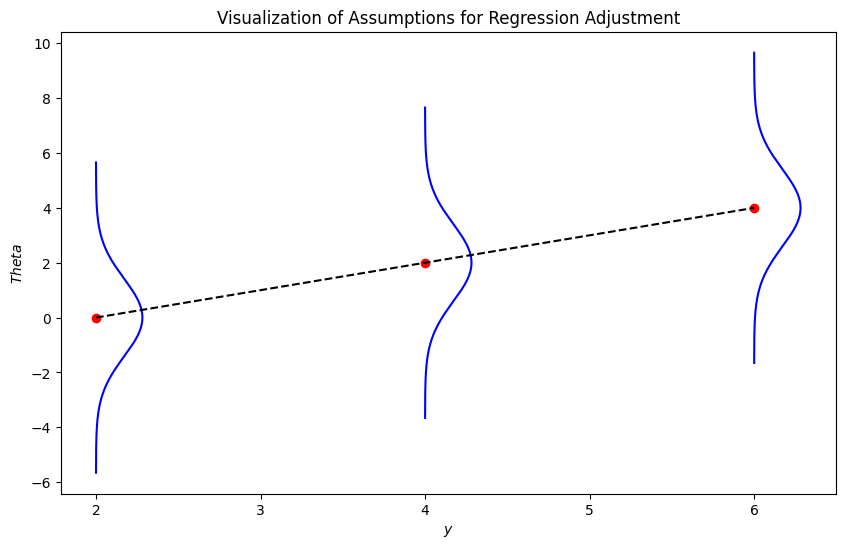
\includegraphics[width=1\linewidth]{overviews//ABC//figures/abc_asummp.png}
\end{figure}

\subsection{Worked Example}
We did this for the Poisson-Gamma posterior. The improvement after regression adjustment is significant. Referring to Figure 10 we see the green dashed line ( $\delta=1$, regression-adjusted) is closer to the posterior than the solid green line (unadjusted) and similarly for the blue lines at $\delta=0.5$.

\begin{figure}
    \centering
    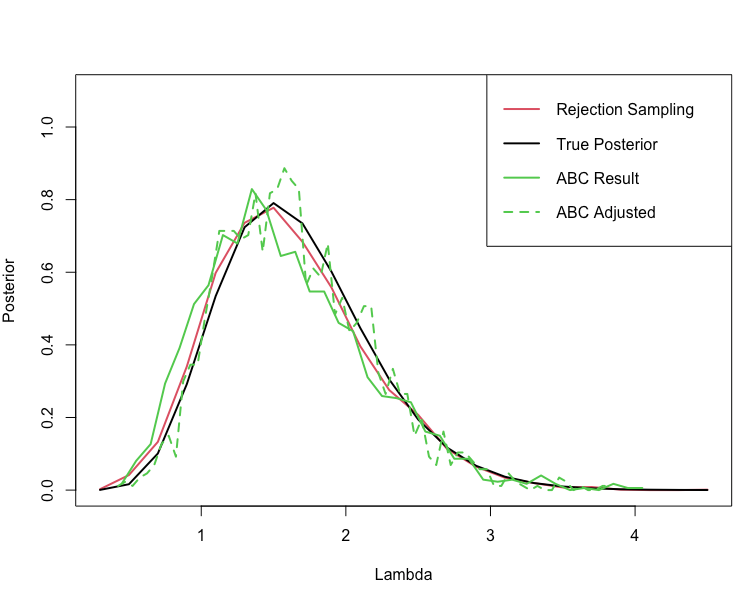
\includegraphics[width=1\linewidth]{overviews//ABC//figures/abc-comps.png}
\end{figure}

\printbibliography


\newpage
\appendix
\section{Code}
\inputminted[linenos=true]{python}{code/abc_assump.py}
\inputminted[linenos=true]{R}{code/abc-comps.R}


\end{document}